\section{Evaluation} \label{sec:eval}

We will evaluate our proposed schemes using a variety of methods as we present below. 
%The evaluation process will demonstrate the feasibility of our research results. 
Our implementation details and source code will be \textit{\ul{publicly available}}.



\paragraph{Simulation-based Evaluation.} All of our approaches will first be evaluated using an \textit{internally developed simulator}. We will use the simulator 
%to analyze the scalability of the algorithms and also 
to test with a more diverse set of real-time task parameters to explore the design-space and scalability of the solutions/algorithms that have been developed. In the past, we extensively use open-source and custom in-house simulators~\cite{sdn_qos_rtss17, sdn_qos_infocom21, sdn_qos_secsdn20, mhasan_rtss16, mhasan_certs16, mhasan_date18, mhasan_twc14_1, mhasan_twc14_2, mhasan_tcom15_1, mhasan_tcom15_2} primarily to test the theories, and we will use similar techniques to evaluate our proposed schemes. 




\paragraph{System Integration and Benchmarks.} We will integrate our proposed ideas into \textit{two real-time kernels} (RT\_PREEMPT~\cite{rt_patch} and LITMUS\textsuperscript{RT}~\cite{litmus_rt}) and use OP-TEE~\cite{optee} as our secure enclave. We will develop kernel patches and evaluate them on both x86 (UP Extreme~\cite{up_extreme}) and ARM (Raspberry Pi~\cite{rpi4}) embedded hardware platforms. We will use existing intrusion detection tools such as Tripwire~\cite{tripwire}, AIDE~\cite{aide}, and Bro~\cite{bro} as security tasks. Further, we will evaluate the efficacy of our scheduler implementations using \textit{three embedded benchmark suites}: PapaBench~\cite{nemer2006papabench}, MiBench~\cite{guthaus2001mibench},  and MultiBench~\cite{eembc_multibench}. These tools and benchmarks will enable us to evaluate the performance of models with realistic workloads. We will use \textit{multiple performance indicators} (such as context switch and memory overheads, scheduling delays) to evaluate the trade-offs of integrating security into existing real-time schedulers.


\begin{wrapfigure}{r}{0.350\textwidth}
	\centering
		\vspace*{-0.3\baselineskip}
%	\hspace*{-1.5em}
	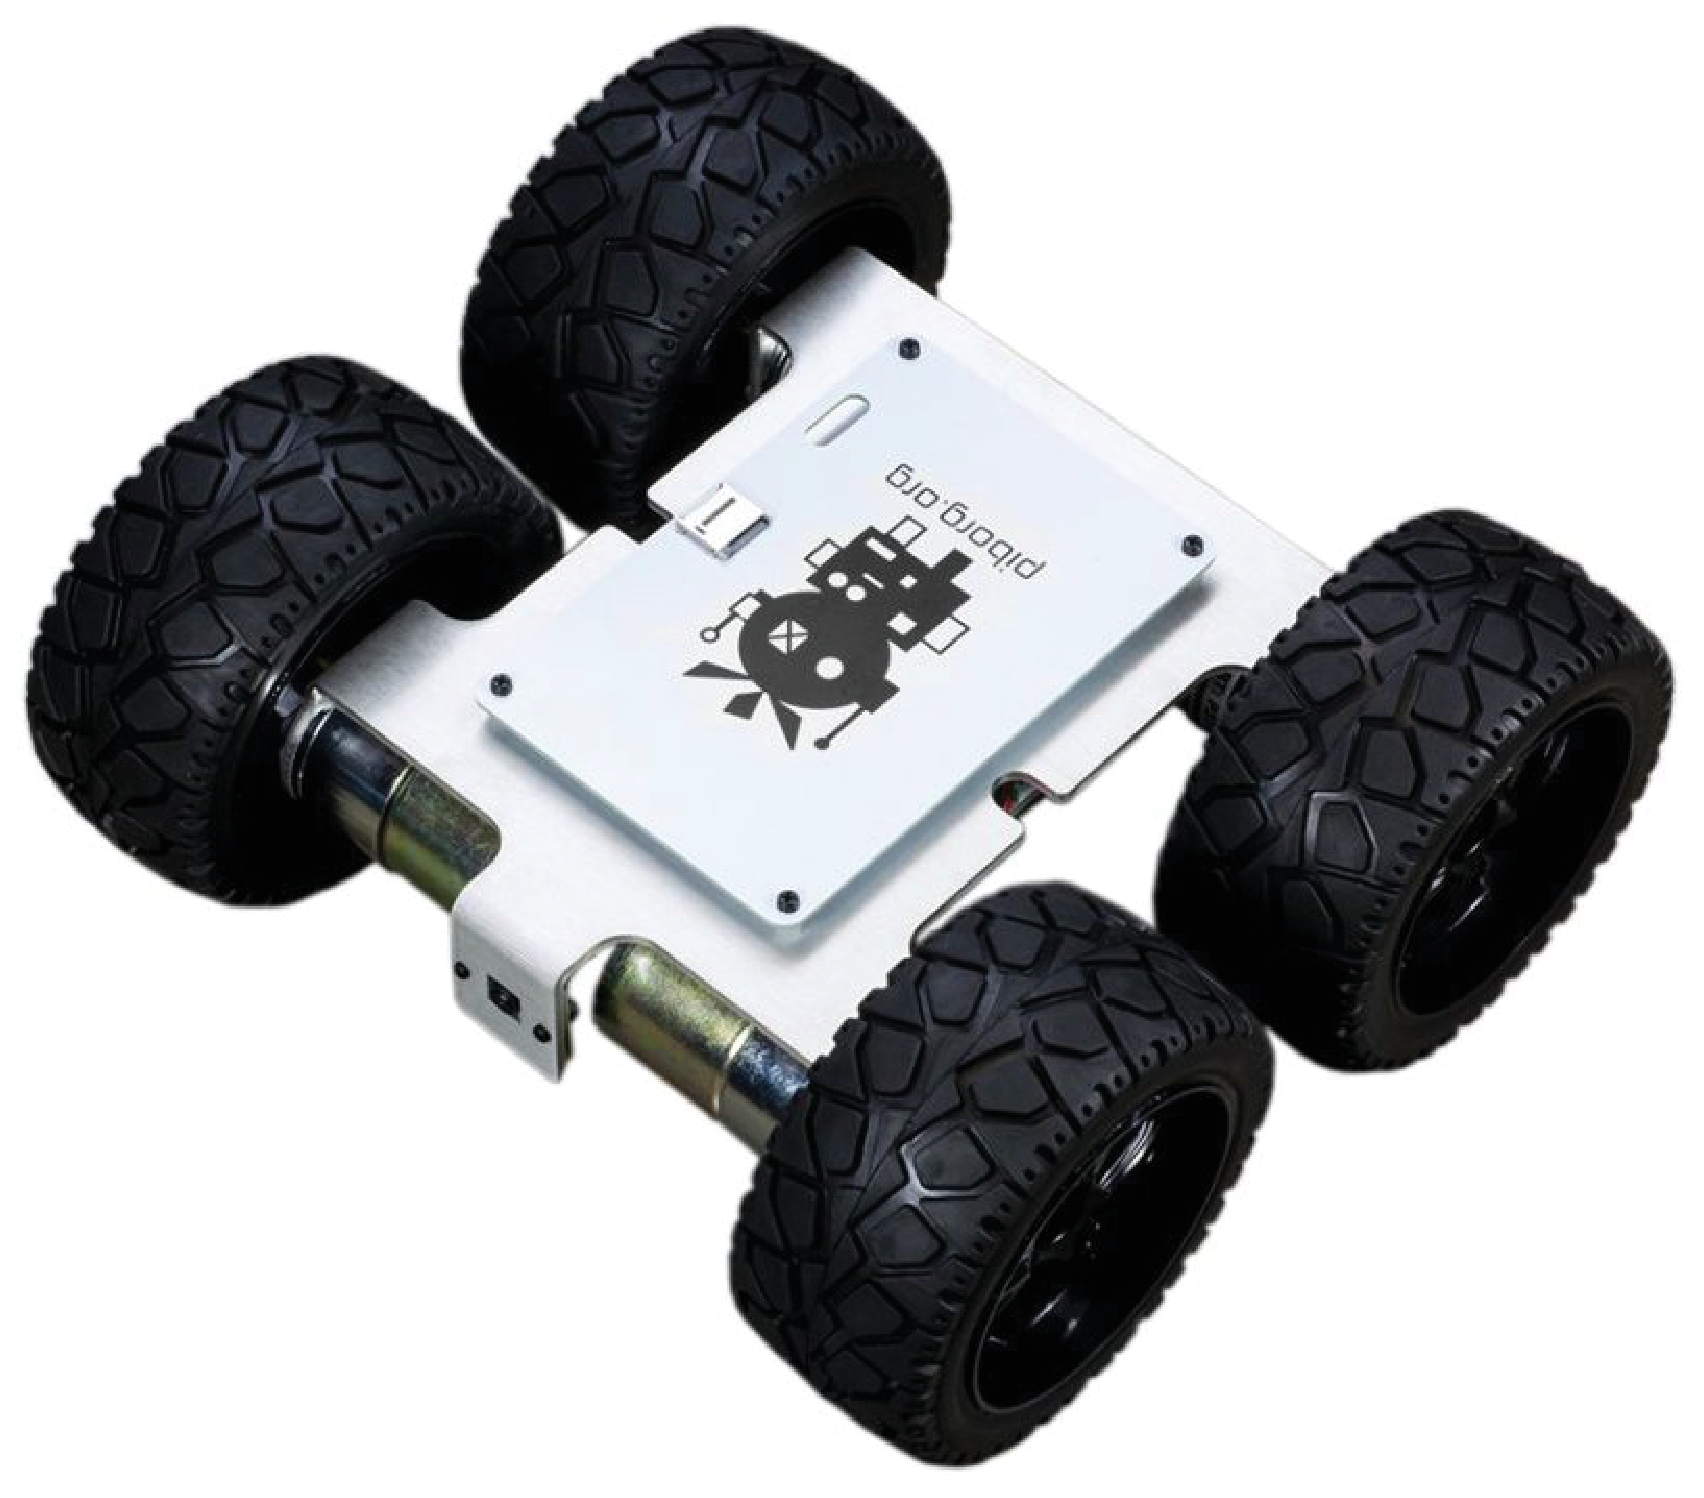
\includegraphics[scale=0.10]{piborg}
	\hspace*{1em}
	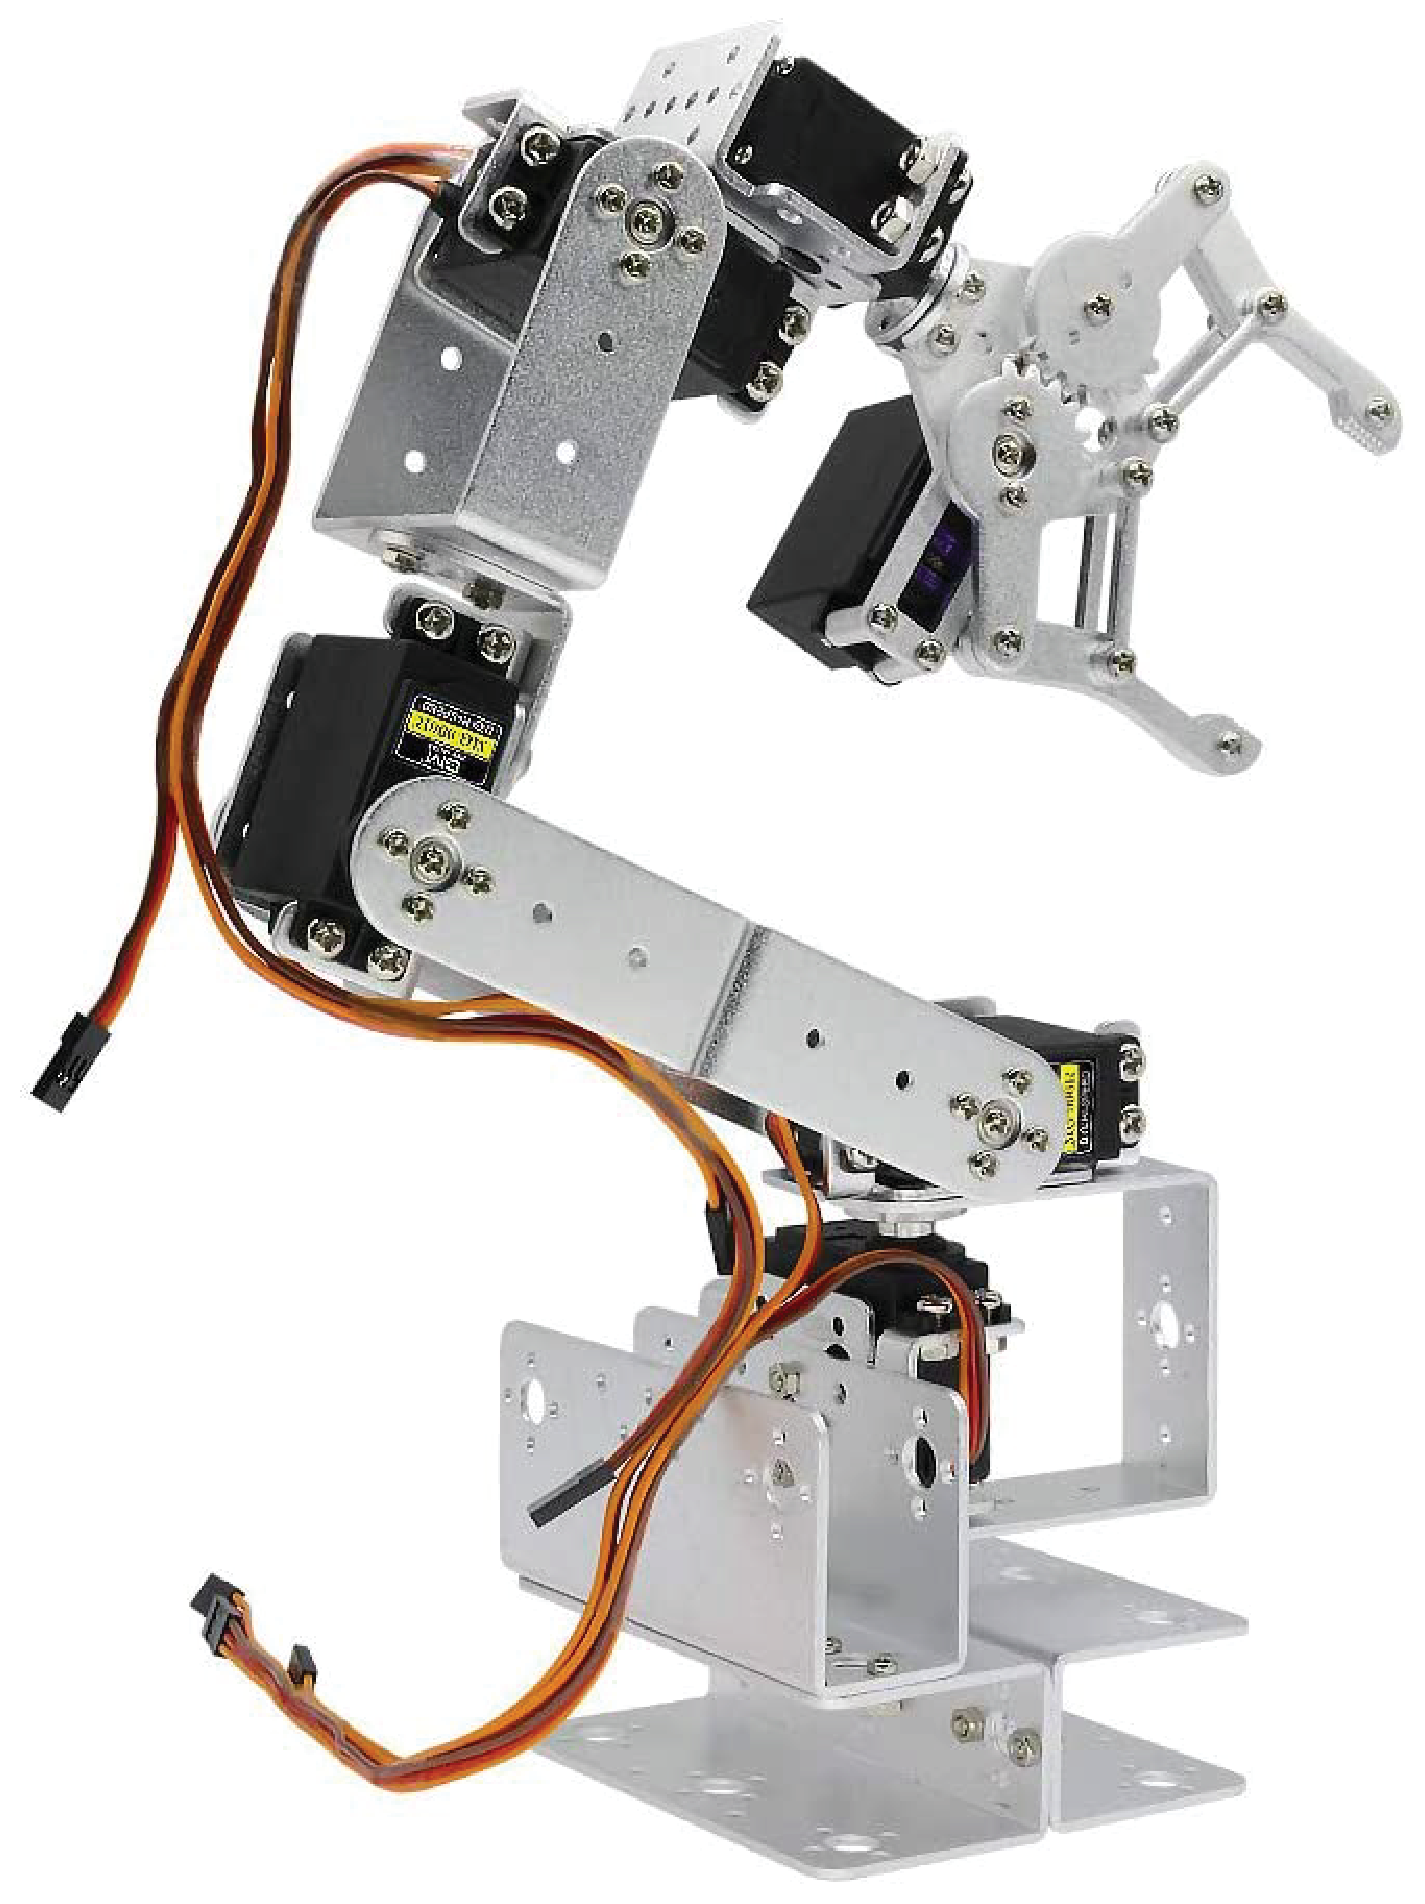
\includegraphics[scale=0.085]{robot_arm}
	%	\includegraphics[scale=0.08]{testbed_piborg}
	%	\includegraphics[scale=0.08]{testbed_robot_arm}
	%	\includegraphics[scale=0.09]{piborg_2_png}
	%	\includegraphics[scale=0.070]{robot_arm_2_png}
	\caption{Off-the-shelf testbeds: \ca multi-terrain rover (left) and \cb six-degree-of-freedom robotic arm (right).}
	\label{fig:demo_sys}
	\vspace*{-0.2\baselineskip}
\end{wrapfigure}


\paragraph{Demonstrative Platforms.} While our simulation-based studies focus on the scalability of the algorithms, we also aim to analyze the feasibility of our ideas in realistic environments. We will evaluate our ideas on \textit{two off-the-shelf cyber-physical platforms} (see Figure~\ref{fig:demo_sys}): \ca a multi-terrain ground rover (MonsterBorg~\cite{monsterborg}) and \cb a six-degree-of-freedom robotic arm (ROT3U~\cite{robot_arm_rot3u}). Our implementations will demonstrate the feasibility of security integration techniques on wide range of use-cases such as remote surveillance, home automation, and smart manufacturing. 

%We will use Raspberry Pi boards to control the hardware platforms and port our RT\_PREEMPT and LITMUS\textsuperscript{RT} scheduler plugins.  

%We will conduct both \textit{\ul{``blue team''} and \ul{``red team''} experiments }
%%to evaluate the efficacy of randomization protocols on our demonstrative platforms 
%where the red team will try to launch side-channel attacks on top of the defense mechanisms integrated by the blue team. The proposed setup will allow us to evaluate the efficacy of randomization protocols on real systems.


